\documentclass{standalone}
\usepackage{tikz}
\usetikzlibrary{automata, positioning, arrows}
\usepackage{amssymb}
\begin{document}
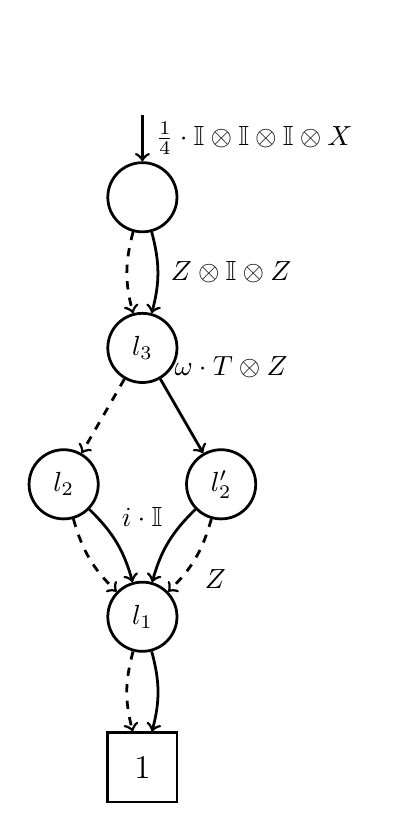
\begin{tikzpicture}[auto,node distance=1.5cm,every node/.style={shape=circle , align=center,solid,minimum size =0.01cm},line width =1pt]
  \tikzstyle{every state}=[fill=white,draw=black,text=black]

  \node[state] (A) {};
  \node[state] (B) [below = 1cm of A] {$l_3$};
  \node[state] (D) at ([shift = ({240:2cm})]B) {$l_2$};
  \node[state] (E) at ([shift = ({-60:2cm})]B) {$l_2'$};
  \node[state] (D1) [below =2.5cm of B] {$l_1$};
  \node[state,shape = rectangle] (T) [below = 1cm of D1] {\large$1$};
  \node[state,draw=none] (I) [above of= A]       {};

  \path[->]
  (A) edge[dashed,bend right=15]  node {} (B)
  (A) edge[bend left=15]  node {$Z\otimes\mathbb{I}\otimes Z$} (B)
  (B) edge[dashed]  node {} (D)
  (B) edge  node {$\omega\cdot T\otimes Z$} (E)
  (D) edge[dashed, bend right = 15] node {} (D1)
  (D) edge[bend left = 15] node {$i\cdot \mathbb{I}$} (D1)
  (E) edge[bend right = 15] node {} (D1)
  (E) edge[dashed, bend left=15] node {$Z$} (D1)
  (D1) edge[bend left = 15] node {} (T)
  (D1) edge[dashed, bend right=15] node {} (T)
  (I) edge node{$\frac{1}{4} \cdot \mathbb{I} \otimes \mathbb{I} \otimes \mathbb{I} \otimes X$} (A);

\end{tikzpicture}
\end{document}